\section*{Segmentation: Generalized Base/bounds}
\begin{minipage}{.6\linewidth}
  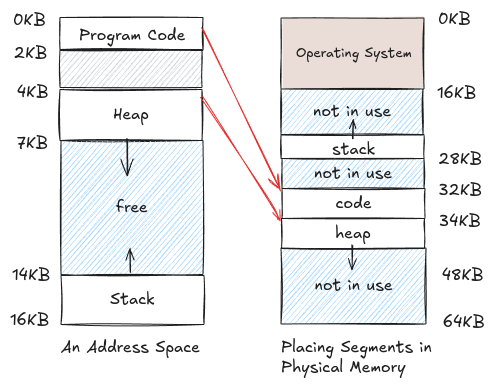
\includegraphics[width=\linewidth]{imgs/addr_map}
\end{minipage}
\begin{minipage}{.4\linewidth}
  \begin{tabular}[th!]{lccl}
    Seg. & Base & Size & Offset\\
    \hline
    Code & 32K  & 2K   & 0     \\
    Heap & 34K  & 3K   & 4K    \\
    Stak & 28K  & 2K   & 16K*   \\
    \hline
    \multicolumn{4}{l}{* stack grows to lower addr} \\
    \hline
  \end{tabular}
  Given addr in the segment:\\
  new = addr \textcolor{err}{-} offset + base
  \begin{itemize}
  \item Addr 100 in code segment:
  \item[] 100 - 0 + 32K = 32868
  \item Addr 4200 in heap segment:
  \item[] 4200 - 4K + 32K = 34920
  \item Addr 7100 $\to$ seg. fault
  \end{itemize}
\end{minipage}
\section*{Segment Reference (explicit approach)}
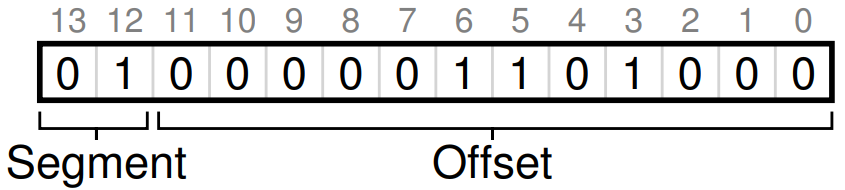
\includegraphics[width=\linewidth]{imgs/explicit2}
\begin{itemize}
\item one segment is unused $\to$ put code in heap to use 1 bit for segment
\item virtual address space is limited to 4KB (max in this example)
\end{itemize}
\section*{Stack and Sharing}
\begin{tabular}[th!]{lcclll}
  Seg. & Base & Size (max 4K) & Offset & Grows pos? & Protection*\\
  \hline
  Code$_{00}$ & 32K  & 2K   & 0    & 1 & Read-Exec  \\
  Heap$_{01}$ & 34K  & 3K   & 4K   & 1 & Read-Write \\
  Stak$_{11}$ & 28K  & 2K   & 16K  & 0 & Read-Write \\
  \hline
  \multicolumn{6}{l}{* protection bits in hardware is to support code sharing} \\
  \hline
\end{tabular}
Virtual addr: 11 1100 0000 0000 $\to$ 15K (0x3c00)
\begin{itemize}
\item 11 $\to$ in stack segment and left 3K (1100 0000 0000)
\item mapped = 3K - 4K (max segment size) + 28K (base) = 27K
\end{itemize}
